\documentclass[twocolumn,aps,prx,amsmath,amssymb,longbibliography]{revtex4-2}
\usepackage{graphicx}
\usepackage{dcolumn}
\usepackage{bm}
\usepackage{amsfonts}
\usepackage{xcolor,tabu}
\usepackage{multirow}
\usepackage{amsthm}
\usepackage{textcomp}
\usepackage{tikz}
\usepackage[colorlinks=true,
            linkcolor=blue,
            urlcolor=blue,
            citecolor=blue]{hyperref}
\hypersetup{bookmarksopen=true}
\usepackage{xr}
% Comment type:
  % -- general comments and communications: questions, uncertainties, marks for further considerations, etc.
  %% -- the original sentence
  %%% -- my changes and reason(s) for the change

% modified sentences will be used in the main text.
% comments will be below the modified sentence

% Things to discuss:

\begin{document}

\title{Density Fluctuations and Energy Spectra of 3D Bacterial Suspensions}

\author{Zhengyang Liu}
%\email{liux3141@umn.edu}
\author{Wei Zeng}
\author{Xiaolei Ma}
\author{Xiang Cheng}
\email{xcheng@umn.edu}


\affiliation{Department of Chemical Engineering and Materials Science, University of Minnesota, Minneapolis, MN 55455, USA}

\date{\today}


\begin{abstract}
We experimentally study density fluctuations and energy spectra of three-dimensional (3D) bacterial suspensions over a wide range of bacterial concentrations. Our results quantitatively verify the predicted scaling law of giant number fluctuations in 3D wet active fluids. Moreover, we show that such a scaling behavior persists at small scales even in low-concentration suspensions well before the transition to bacterial turbulence. Our measurements on the energy spectra of bacterial suspensions support the theoretical prediction on the flow of dilute pusher swimmers and reveal the characteristic turbulent energy spectra of dense bacterial suspensions in the bulk limit. Lastly, we also examine the density-flow coupling in both the steady and transient states of active turbulence. A universal density-independent and scale-invariant correlation between giant number fluctuations and energy spectra is found across multiple length scales. Our systematic experiments verify important theoretical predictions on density fluctuations and turbulent flow structures of 3D wet active fluids and provide new insights into the emergent dynamics of bulk bacterial suspensions.

\end{abstract}

\maketitle

\section{introduction}

Active fluids exhibit many unusual behaviors beyond the expectation of equilibrium statistical mechanics \cite{Ramaswamy2010,Cates2012,Marchetti2013,Poon2013,Elgeti2015}.
In particular, an active fluid can exhibit anomalously large density variations, the so-called giant number fluctuations (GNF), where the standard deviation of the number of particles $\Delta N$ grows nonlinearly with the square root of the mean particle number $\sqrt N$, defying the central limit theorem of equilibrium systems \cite{Mishin2015}.
Such unusual density fluctuations have been observed in a wide range of active fluids in both living and non-living systems including vibrated granular rods \cite{Narayan2007,Aranson2008,Kudrolli2008,Deseigne2010}, swarming bacteria \cite{Zhang2010,Nishiguchi2017} and mammalian cells \cite{Kawaguchi2017},
self-propelled cytoskeleton \cite{Schaller2013}, and synthetic colloidal swimmers \cite{Palacci2013,Karani2019}. Hence, GNF is generally viewed as a hallmark of the emergent behaviors of active fluids.


Although significant progress has been made in the theoretical understanding of GNF over the past two decades \cite{Toner1995, Tu1998, Toner1998, AditiSimha2002, Ramaswamy2003, Toner2005, Chate2008, Mishra2010, Dey2012, Saintillan2012, Saintillan2013, Ngo2014,  Mahault2019}, systematic experiments that can quantitatively verify theoretical and numerical predictions are still few and far between. Particularly, the existing experiments on GNF all focused on dry two-dimensional (2D) or quasi-2D systems \cite{Narayan2007, Aranson2008, Kudrolli2008, Deseigne2010, Zhang2010, Schaller2013, Nishiguchi2017, Kawaguchi2017, Palacci2013}, where particle-boundary interactions play a significant role in affecting the density fluctuations of 2D active fluids \cite{Marchetti2013}. Such system-specific interactions lead to a variety of scaling behaviors in GNF defined via $\Delta N/\sqrt N \sim N^\alpha$. A wide range of the scaling exponent $\alpha$ between 0.13 and 0.5 has been reported in different 2D experiments. In comparison, measurements of GNF in wet 3D active fluids, where hydrodynamics dominate the interparticle interactions and conserve the total momentum of systems, have not been achieved heretofore. As a result, experimental verification of the prediction of GNF in 3D wet active fluids without the influence of system boundaries is still out of reach. Important questions such as how the long-ranged hydrodynamic interactions and the dimensionality of systems affect the density fluctuations of active fluids have not been properly addressed in experiments.




%% Although significant progress has been made in the theoretical understanding of GNF over the last two decades since the seminal works of Toner and Tu\cite{Toner1995,Tu1998,Toner1998,AditiSimha2002,Ramaswamy2003,Toner2005,Chate2008,Mishra2010, Dey2012,Saintillan2012,Saintillan2013,Ngo2014,Mahault2019}, quantitative experimental verification of many important theoretical and numerical predictions on GNF is still out of reach. Of particular interest is the scaling exponent $\alpha$, which is defined following $\Delta N /\sqrt N \propto N^\alpha$, where $\Delta N$ is the standard deviation of particle number and $N$ is the mean number of particles in a subsystem of given size. Heretofore, all the existing experiments on GNF were limited to two-dimensional (2D) or quasi-2D systems. In contrast to theoretical predictions (where $\alpha \approx 0.3$), $\alpha$'s obtained in these experiments show large variations ranging from 0.13 to 0.5. Such a large variation arises partially because of complicated particle-boundary interactions, which are hard to incorporate in theoretical studies. Moreover, the predictions of $\alpha$ in three-dimensional (3D) wet active fluids---one of the most important classes of active fluids where hydrodynamics dominate the interparticle interactions and conserve the total momentum of systems \cite{Marchetti2013}---has not been experimentally testified. Therefore, there is an imperative need for an experimental measurement of $\alpha$ in 3D active fluids, which are not affected by system boundaries. Such a measurement will provide not only an unambiguous experimental benchmark to testify theories of active fluids, but also experimental support on the effect of dimensionality on GNF of active fluids \cite{Marchetti2013}.

The rise of GNF in active fluids is usually accompanied by the transition to ordered phases with collective motion \cite{Ramaswamy2010,Marchetti2013}. For wet 3D active fluids such as bacterial suspensions, the collective motion lead to large-scale coherent flows with intermittent vortices and jets, which are often referred to as active turbulence \cite{Wolgemuth2008,Wensink2012,Dunkel2013a,Bratanov2015,Guo2018,Linkmann2019,Bardfalvy2019,Alert2020,Skultety2020,Peng2020}. Similar to GNF that manifests density fluctuations across different scales, the flow of active turbulence also exhibits scale-dependent structures. Imported from the study of classical turbulence, energy spectra are frequently used to quantify such scale-dependent structures in active turbulence \cite{Ishikawa2011,Wensink2012,Dunkel2013a,Giomi2015,Creppy2015,Patteson2018,Alert2020}. Nevertheless, current experimental studies of energy spectra were limited to active turbulence at high particle concentrations. A systematic measurement of energy spectra over a broad range of particle concentrations is still lacking. More importantly, although both GNF and energy spectra quantify the scale-dependent dynamics of active fluids, the intrinsic connection between these two quantities across different scales has not been investigated.


\begin{figure}[t]
	\begin{center}
		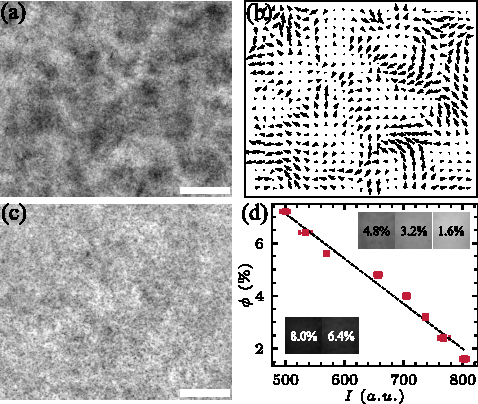
\includegraphics[width=0.47\textwidth]{Figures/experiment/v5.pdf}
		\caption[Experimental details]
		{Density fluctuations and active turbulence.
			(a) A snapshot of a dense suspension of \textit{E. coli} with bacterial volume fraction $\phi = 6.4\%$.
			(b) 2D velocity field of the suspension shown in (a), which exhibits characteristic active turbulent flow patterns.
			(c) A snapshot of a dilute suspension of \textit{E. coli} with $\phi = 1.6\%$, which shows no active turbulent flows. Scale bars are 85 $\mu$m.
			(d) Average pixel intensities of images, $I$, as a function of $\phi$. Inset shows the images of bacterial suspensions of different $\phi$ under the same light illumination.
		}
		\label{fig:experiment}
	\end{center}
\end{figure}

Here, we present our systematic experimental study of GNF and energy spectra in bulk bacterial suspensions, a premier example of 3D wet active fluids \cite{Marchetti2013}. Our experiments on GNF in high-concentration bacterial suspensions quantitatively verify the theoretical prediction on the scaling behavior of density fluctuations in 3D wet active fluids. More surprisingly, we find that such a scaling relation persists at small scales even in low-concentration suspensions well below the transition to bacterial turbulence. Such an unusual behavior arises due to the long-range nature of hydrodynamic interactions, lacking in 2D dry systems. Our systematic measurements on the energy spectra of bacterial suspensions of different concentrations further illustrate the emergence of the characteristic flow structure of active turbulence and verify the prediction of the energy spectra of dilute pusher suspensions. Lastly, our experiments also reveal a density-independent and scale-invariant coupling between GNF and energy spectra. Quantitatively similar coupling has also been uncovered in the kinetic process during the transition towards bacterial turbulence. Taken together, our study provides a solid experimental benchmark on density fluctuations and energy spectra of 3D bacterial suspensions and reveals an unexpected coupling between GNF and energy spectra across multiple length scales. As such, our experiments provide not only the first verification on several important theoretical predictions including the scaling law of GNF in wet 3D active fluids, the energy spectra of uncorrelated pusher swimmers and the delayed onset of density fluctuations, but also new insights into the emergent dynamics of bulk bacterial suspensions such as local bacterial correlation in dilute suspensions and the universal coupling between density fluctuations and flow energies in the steady and transient states of active turbulence.
% \textcolor{red}{Bridging these two different aspects of active fluids provides new insights into the origin of GNF and reveal hidden dynamic structures of active turbulence.}
% Ths significance statement need further modification

%% frequently measured to quantify such scale-dependent flow properties and to illustrate energy transfer between different scales in active turbulence.
%% Nevertheless, existing experiments on energy spectra of active turbulence all focused on high-concentration suspensions with fully developed active turbulent flows \cite{Ishikawa2011,Wensink2012,Dunkel2013a,Creppy2015,Patteson2018}. How the characteristic turbulent spectrum emerges with increasing particle concentration has not been systematically studied.
%% More importantly, although both GNF and energy spectra quantify the scale-dependent dynamics of active fluids, the intrinsic relation between the two quantities have not been explicitly discussed.



\section{Experiment}

We use genetically engineered light-powered \textit{Escherichia coli} (\textit{E. coli}) as our model bacteria \cite{Liu2020}.
% \textcolor{red}{Some details about the light-control bacteria and the culturing procedure needed to be given in SM.}
For a typical experiment, a bacterial suspension of control volume fraction $\phi$ is injected into a sealed chamber of 20 mm $\times$ 3 mm $\times$ 140 $\mu$m. We calculate $\phi = n V_b$, where $n$ is the number density of bacteria and $V_b = \pi (w_b/2)^2 l_b = 1$ $\mu$m$^3$ is the average volume of a bacterium, where $l_b = 3$ $\mu$m and $w_b = 0.65$ $\mu$m are the average length and width of bacterial body. The volume of bacterial flagella is too small to affect the volume of bacteria.
Without supply of oxygen, bacteria quickly consume all the oxygen in the chamber and stop moving after $5$ minutes.
We then illuminate the suspension with a high-intensity microscope light, which powers bacteria at their maximal swimming speed of $v_0 = 15 \pm 3$ $\mu$m/s in the dilute limit.
A video of the suspension is taken 50 $\mu$m above the bottom wall of the chamber by a bright-field inverted microscope at a frame rate of $30$ fps with the field of view of $420 \times 360$ $\mu$m$^2$ (Fig.~\ref{fig:experiment}a).
We use a standard Particle Image Velocimetry (PIV) algorithm \cite{Liberzon2020} % cite openPIV package
to extract the 2D in-plane velocity field $(v_x,v_y)$ in the 3D suspension. The suspension exhibits the characteristic chaotic vortices and jets of active turbulence at high $\phi$ (Fig.~\ref{fig:experiment}b).

It is challenging to directly count the number of bacteria in a 3D dense suspension of fasting moving bacteria. Luckily, by virtue of Beer-Lambert law, the local bacterial density is monotonically correlated with the local intensity of microscope images, where darker regions correspond to higher bacterial densities (Fig.~\ref{fig:experiment}a, c and Supplementary Video). Such a principle has already been exploited in previous experiments in probing the dynamics of bacterial suspensions and actin filaments \cite{Sokolov2009, Wilson2011, Schaller2013}. To calibrate the density-intensity correlation, we prepare bacterial suspensions of different $\phi$ and image the suspensions under the same illumination (Fig.~\ref{fig:experiment}d inset). The mean image intensity decreases with increasing $\phi$ following an approximately linear relation (Fig.~\ref{fig:experiment}d), agreeing with the the Beer-Lambert law for samples of small thickness and weak absorptivity appropriate for our experiments. The linear density-intensity relation has also been used in previous experiments on \textit{E. coli} suspensions \cite{Wilson2011}.


\begin{figure}[ht]
\begin{center}
\includegraphics[width=0.47\textwidth]{figures/spatiotemporal-correlations/v5.pdf}
\caption[spatiotemporal-correlations.]
{
Density and velocity spatiotemporal correlations. (a) Two-point density correlations at different bacterial volume fractions $\phi$. Radial position $r$ is normalized by the average length of bacteria $l_b = 3$ $\mu$m. (b) Density autocorrelations at different $\phi$. Time $t$ is normalized by the characteristic swimming time of bacteria $\tau_b = 0.2$ s. (c) Two-point velocity correlations at different $\phi$. (d) Velocity autocorrelations at different $\phi$. $\phi$ ($\%$) of different curves are indicated in (a). (e) Correlation lengths of density and velocity, $\lambda$, versus $\phi$. (f) Correlation times of density and velocity, $\tau$, versus $\phi$.
}
\label{fig:spatiotemporal-correlations}
\end{center}
\end{figure}

\begin{figure}[ht]
\begin{center}
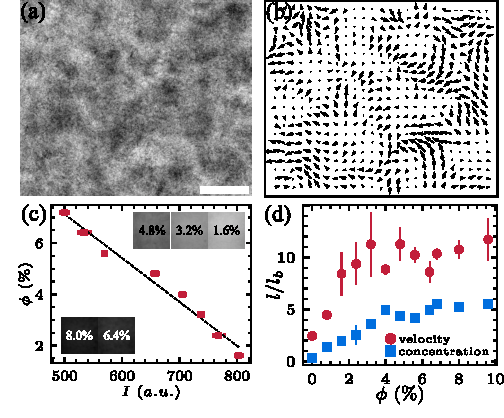
\includegraphics[width=0.47\textwidth]{figures/GNF/v4.pdf}
\caption[Concentration dependence of GNF.]
{
Giant number fluctuations (GNF) for suspensions of different volume fractions $\phi$. The standard deviation of particle number $\Delta N$ normalized by the square root of the mean number of particles $\sqrt N$ as a function of the scaled subsystem size $l^2/l_b^2$. Black dashed line indicates the density correlation lengths $\lambda(\phi)$ (see Fig.~\ref{fig:spatiotemporal-correlations}e). Black dashed line indicate a power-law scaling of 0.33. \textcolor{red}{Please add the symbol for $\phi=0$ in the legend. As we have discussed, change the black line to symbols for $\lambda(\phi)$.} Inset: Scaling exponent $\alpha$ versus $\phi$. $\alpha$ are extracted by fitting the experimental data from 0.3$l_b$ to $\lambda(\phi)$. The dashed line in the inset indicates the theoretical prediction of $\alpha=0.33$.
}
\label{fig:GNF}
\end{center}
\end{figure}

\section{Results}

\subsection{Density fluctuations}

The simple linear relation allows us to measure the spatiotemporal evolution of local bacterial densities and investigate density fluctuations in 3D bacterial suspensions. We first calculate the two-point density spatial correlation, $C_n$, and the density auto-correlation, $C_{t,n}$, for suspensions of different $\phi$ (Fig.~\ref{fig:spatiotemporal-correlations}a, b) and compare them with the well-studied velocity correlations, $C_{v}$ and $C_{t,v}$, extracted from PIV (Fig.~\ref{fig:spatiotemporal-correlations}c, d).

The correlation length $\lambda$ and correlation time $\tau$ are determined when the corresponding normalized correlation functions decay to $1/e$ (Fig.~\ref{fig:spatiotemporal-correlations}e, f). Figure~\ref{fig:spatiotemporal-correlations}e shows the density correlation length $\lambda$ at different $\phi$, which quantifies the scale of density inhomogeneities in suspensions.
$\lambda$ is small at low $\phi$, gradually increases with $\phi$ and reaches a plateau of $\sim 5l_b$ in high-concentration bacterial suspensions when $\phi > \phi_c = 3.5\%$. \textcolor{red}{Is $\phi_c$ the transition concentration to active turbulence?} The velocity correlation length follows a qualitatively similar trend and also saturates above $\phi_c$, consistent with previous finding \cite{Sokolov2007}. The saturated velocity correlation length is about twice of the saturated density correlation length, which is determined by the size of system \cite{Guo2018}.  Figure~\ref{fig:spatiotemporal-correlations}f further compares the density and velocity correlation times, $\tau$, at different $\phi$. Although the density and velocity correlation times at low $\phi$ show a large discrepancy, they both plateau when $\phi > \phi_c$ at $\sim 5\tau_b$, where $\tau_b=l_b/v_0=0.2$ s is the characteristic swimming time scale of \textit{E. coli}. The saturated velocity correlation time is slightly larger than the saturated density correlation time. The similarity between the density and the velocity correlation functions at high $\phi$ indicates a strong coupling between density fluctuations and active turbulent flows, a feature we shall
examine in more details in Sec.~\ref{Density-flow coupling} across different length scales.
% I don't know how to interpret the large difference in \tau at low concentration. It may be due to the dominanace of illumination light at low concentration.

We further examine GNF by calculating the standard deviation of bacterial number $\Delta N$ and the mean bacterial number $N$ in subsystems of increasing sizes \cite{Liu2020}. $\Delta N / \sqrt N$ as a function of $l^2/l_b^2$ for bacterial suspensions of different $\phi$ is plotted in Fig.~\ref{fig:GNF}, where $l$ is the side length of square subsystems. Note that since the depth of field of our images is fixed, the area of the subsystem $l^2$ is linearly proportional to the average number of particles $N$ in the subsystem at a fixed $\phi$. At a given $\phi$, $\Delta N/\sqrt N$ plateaus when $l$ is significantly larger than the density correlation length at the corresponding $\phi$, $\lambda(\phi)$ (Fig.~\ref{fig:spatiotemporal-correlations}e). The central limit theorem applies at large length scales owing to the spatial average over multiple dense and dilute regions. Nevertheless, at small length scales when $l$ is comparable or smaller than $\lambda(\phi)$, bacterial suspensions of all $\phi$ in our study exhibit obvious GNF, where $\Delta N/\sqrt N$ increases with increasing subsystem size. More remarkably, $\Delta N/\sqrt N$ versus $l^2$ approaches the same scaling in the small $l$ limit even for low-$\phi$ suspensions without turbulent flows. Such a surprising finding is in sharp contrast to GNF of 2D active systems, where GNF gradually diminishes with decreasing particle density \cite{Narayan2007,Aranson2008,Kudrolli2008,Deseigne2010,Zhang2010,Schaller2013}. Kinetic theories have predicted that, due to the long-range hydrodynamic interactions, pusher-type microswimmers in 3D active suspensions show strong spatial and temporal correlations at low concentrations well below the transition concentration to active turbulence \cite{Stenhammar2017,Nambiar2021}. Although the original theories discussed the effect of the correlation on the enhanced diffusion of passive tracers and velocity fluctuations in dilute suspensions, our experiments show that such a correlation also manifests as GNF at small length scales in low concentration bacterial suspensions.


Quantitatively, the strength of GNF can be measured by the scaling exponent $\alpha$ following $\Delta N/\sqrt{N} \sim N^\alpha$. $\alpha=0$ for equilibrium systems obeying the central limit theorem, whereas the upper bound $\alpha = 0.5$ corresponds to a system with maximal density fluctuations.
We extract $\alpha$ by fitting the experimental curves with the power-law relation for $l < \lambda(\phi)$. The inset of Fig.~\ref{fig:GNF} shows $\alpha$ as a function of $\phi$, where $\alpha$ remains approximately constant at $0.30 \pm 0.03$ for all $\phi$. In contrast, $\alpha$ decreases continuously with decreasing $\phi$ for 2D GNF. Notably, for high $\phi \geq XX\%$, $\alpha$ approaches a narrower plateau of $0.33 \pm 0.01$, quantitatively agreeing with the theoretical prediction of $\alpha = 1/3$ for 3D suspensions of polar-ordered self-propelled particles with hydrodynamic interactions \cite{AditiSimha2002}. Hence, our experiments quantitatively verify the theory of the GNF of 3D wet active fluids. More interestingly, our study shows that the same GNF scaling persists in low concentration suspensions at small scales even before the emergence of the polar order of bacteria at large scales.

\begin{figure}[!]
\begin{center}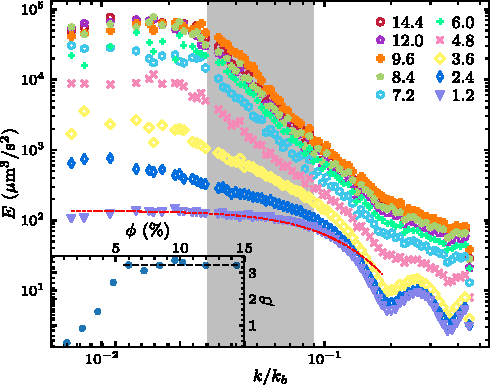
\includegraphics[width=0.47\textwidth]{Figures/energy-spectra/v4.pdf}
\caption[Concentration dependence of energy spectra.]
{
Energy spectra $E(k)$ of bacterial suspensions of different volume fractions $\phi$. Shaded region indicates the range over which the scaling exponent $\beta$ is fitted. Red dashed line is a fitting of $E(k)$ at $\phi=XX\%$ using Eq.~\ref{eq:energy-spectra}. The bacterial number density $n=\phi V_b$ and the dipole length $l_d = 1.9$ $\mu$m are from experiments (see text), whereas \textcolor{red}{the dipole strength $\kappa = XX$ $\mu$m$^3$/s and the regularization length $\epsilon = XX$ $\mu$m are taken as fitting parameters.}
Inset: Scaling exponent of $E(k)$, $\beta$, as a function of $\phi$. Dashed line indicates $\beta = 3.3$. \textcolor{red}{The text gives 3.2 instead of 3.3.}.
}
\label{fig:energy-spectra}
\end{center}
\end{figure}

\subsection{Energy spectra}

Similar to GNF, the velocity field of active turbulence also shows scale-dependent structures, which are often characterized by the energy spectrum of turbulent flows, $E(k)$ \cite{Liu2020}. $E(k)$ measures the kinetic energy density at different scales in terms of wavenumber $k = 2\pi/l$. It is related to the mean kinetic energy density $E = \langle v_x^2 + v_y^2 \rangle/2$ via $E = \int_0^\infty E(k)dk$. Figure~\ref{fig:energy-spectra} shows $E(k)$ of bacterial suspensions at different $\phi$. $E(k)$ of low-$\phi$ suspensions with uncorrelated pusher swimmers has been predicted \cite{Bardfalvy2019}
\begin{equation}
\label{eq:energy-spectra}
E(k) = 4\pi n \kappa^2 \left[ \frac{1}{3} + \frac{\cos(kl_d)}{(kl_d)^2} - \frac{\sin(kl_d)}{(kl_d)^3} \right] \frac{\epsilon^4k^2}{l_d^2} K_2^2(k\epsilon),
\end{equation}
where $n$ is the number density of bacteria, $\kappa$ is the dipole strength and $l_d$ is the dipolar length of \textit{E. coli}. $\epsilon$ is the distance for the regularization of the dipolar flow field. $K_2$ is the modified Bessel function of the second kind.
The fitting of Eq.~\ref{eq:energy-spectra} agrees well with our experimental $E(k)$ at low $\phi$ in the small $k$ limit (Fig.~\ref{fig:energy-spectra}). Particularly, Eq.~\ref{eq:energy-spectra} dictates that $E(k)$ is flat as $k \to 0$, a key feature of the theory confirmed by our experiments. A simple dimensional analysis can show that the plateau $E(k)$ at the small $k$ follows $\lim_{k \to 0}E(k) \sim n \kappa^2$ for uncorrelated swimmers of density $n$. The dipole strength can be estimated as $\kappa = Fl_d/\eta = \xi v_0 l_d/\eta$, where $\eta$ is the viscosity of the buffer. $\xi$ is the drag coefficient of a bacterial body orientated along its major axis, which can be calculated based on the body geometry $\xi = 3\pi\eta w_b \left[1-(1-l_b/w_b)/5\right]$ \cite{Magariyama2002}. $l_d = 1.9$ $\mu$m from direct measurements \cite{Drescher2011}. Thus, $\lim_{k \to 0}E(k) = 7 \times 10^2$ $\mu$m$^3$/s, within the same order as our experiments. The discrepancy between Eq.~\ref{eq:energy-spectra} and experiments at large $k$ may arise from the correlation between bacteria at small length scales as shown by density fluctuations, as well as PIV errors due to the small number of bacteria in each PIV box of low-$\phi$ suspensions.

With increasing $\phi$, $E(k)$ at small $k$ increases sharply. In the turbulent regime at high $\phi$, the kinetic energy is concentrated at scales much larger than the size of single bacteria, even though the turbulent flow is entirely driven by the swimming of single bacteria. The overall trend of $E(k)$ with increasing $\phi$ qualitatively agrees with the results from large-scale particle simulations \cite{Saintillan2012,Bardfalvy2019}.

We also extract the scaling exponent $\beta$ of $E(k) \sim k^{-\beta}$ by fitting the energy spectra at intermediate $k$, where a significant change of $E(k)$ with $\phi$ occurs and $E(k)$ exhibits good power-law relations. $\beta$ increases with $\phi$ and saturates at $3.2 \pm 0.1$ at high $\phi \geq XX\%$. The saturated scaling exponent is quantitatively similar to that obtained from the active turbulence of high-concentration sperm suspensions at large $k$ \cite{Creppy2015}.
The exponent is also consistent with experiments on confined dense suspensions of \textit{B. subtilis}, where the scaling of $E(k) \sim k^{-8/3}$ has been reported at large $k$ \cite{Wensink2012}.
Since the characteristic turbulent vortex size quantified by the velocity correlation length is linearly proportional to the system size $L$ \cite{Guo2018}, when $k$ is significantly smaller than $2\pi/L$, $E(k)$ would decreases, exhibiting the non-monotonic trend shown in \cite{Wensink2012}. The large system size of $L = 140$ $\mu$m of our experiments allows us to probe the small $k$ limit predicted by theories and simulations without the influence of system boundaries.

Although the scaling in the small $k$ limit is strongly affected by the system size, the scaling in the large $k$ limit seems to be universal with $\beta \approx 3$ from different experiments. To the best of our knowledge, no theoretical prediction has been made on this universal scaling behavior for 3D active turbulence. Giomi investigated the energy spectra of 2D active nematics by combining numerical simulations with mean-field theories and showed $E(k) \sim k^{-4}$ in the large $k$ limit \cite{Giomi2015}.
The result has also been confirmed recently by a hydrodynamic theory \cite{Alert2020}. For isotropic turbulence in $d$ dimension, the energy spectra can be written as $E(k) = C_d k^{d-1} \langle \mathbf{v}(\mathbf{k})\cdot \mathbf{v}(-\mathbf{k})\rangle_{k = |\mathbf{k}|}$ \cite{Wensink2012,Bardfalvy2019},
where $C_d k^{d-1}$ is the surface area of $d$-sphere and $\langle \mathbf{v}(\mathbf{k})\cdot \mathbf{v}(-\mathbf{k})\rangle_{k = |\mathbf{k}|}$ is the Fourier transform of the velocity-velocity spatial correlation function. If the velocity correlation function for 2D active nematics is qualitatively similar to that of 3D bacterial suspensions independent of the dimensionality of systems, the mean-field theory would then predict a scaling of $E(k) \sim k^{-3}$, consistent with experimental observations. Such a hypothesis, although intriguing, is certainly non-trivial and needs further theoretical investigation. Note that although we measure the energy spectra of 2D in-plane flows of 3D suspensions, the scaling of the spectra is determined by the spectra of 3D turbulent flows \cite{Pope2000}. Taken together, our study provides systematic experiments on the evolution of $E(k)$ over a large range of $\phi$ in bulk bacterial suspensions. The results verify the existing theory on low-concentration active pusher suspensions and serve as a benchmark for future theoretical development on the spectral properties of 3D active turbulence.

\begin{figure}[!]
\begin{center}
\includegraphics[width=0.47\textwidth]{figures/GNF-energy-spectra-correlation/v5.pdf}
\caption[The correlation between GNF and kinetic energy and kinetic energy spectra.]
{
Coupling between density fluctuations and kinetic energies.
(a) Energy spectra $E(k)$ plotted against number density fluctuations $\Delta N/\sqrt N$ at each corresponding length scale for bacterial suspensions of different volume fractions $\phi$. Gray symbols are used for low-$\phi$ suspensions without active turbulence. Black dashed line is a polynomial fitting of the master curve, serving as guide for the eye. Black arrow indicates the direction of increasing lengths.
(b) Correlation of local density fluctuations and kinetic energies $C$ as a function of $\phi$. Inset: snapshots of a density fluctuation field and a kinetic energy field for a bacterial suspension of \textcolor{red}{$\phi = XX\%$}.
}
\label{fig:GNF-energy-spectra-correlation}
\end{center}
\end{figure}

\subsection{Density-flow coupling} \label{Density-flow coupling}

Both GNF and energy spectra probe the scale dependence of active bacterial suspensions. The former measures density fluctuations at different scales, whereas the latter considers the transfer of flow energies across scales. Although both properties have been extensively studied, a direct correlation between the two has not been explicitly examined heretofore. Indeed, the quantitative similarity between the density spatiotemporal correlations and the velocity spatiotemporal correlations shown in Fig.~\ref{fig:spatiotemporal-correlations} has already indicated a strong density-flow coupling in the turbulent regime. Moreover, the trends of GNF and energy spectra also show similar characteristics, both exhibiting a rapid increase at small length scales and plateaus at large length scales (Figs.~\ref{fig:GNF} and \ref{fig:energy-spectra}). Such a similarity further suggests that a density-independent correlation between density fluctuations and kinetic energies may exist across all different length scales. To verify the hypothesis, we plot density fluctuations $\Delta N/\sqrt N$ against the corresponding kinetic energies $E$ at the same scale in Fig.~\ref{fig:GNF-energy-spectra-correlation}a. We find that all the $\Delta N/\sqrt N$-$E$ pairs fall onto a universal curve over two orders of magnitude in scales extending from the size of single PIV boxes up to the density correlation length in the turbulent regime, regardless of the specific volume fractions of the samples.
In comparison, $\Delta N/\sqrt N$-$E$ shows much larger scattering for low $\phi$ suspensions without active turbulence.
%% this is a discussion
%% The length scale I plot the coupling is from 10 to 30 um, from smallest PIV box to the length of vortex size. Plotting larger range is possible, but shows larger deviation. Prepare a figure for comparison (GNF-figures slides)
Although it is not surprising that density fluctuations should correlate with kinetic energies in general as both measure different aspects of the same active turbulence, the collapse of data from samples of different volume fractions
% and the constant ratio of $\alpha/\beta$ are
is quite unexpected.
The results show that the coupling between density fluctuations and turbulent flows occur at every scale of active turbulence in a quantitative same fashion. Such a scale-invariant coupling is independent of the volume fraction of bacterial suspensions.
%% and manifests even in the turbulent regime between $\phi_c$ and $\phi_h$ where the linear theory fails.
\textcolor{red}{Since Newtonian fluids are generally considered to be incompressible, this scale-invariant density-flow coupling does not have an analogue in classical turbulence and is unique to active turbulence. I am curious why you don't like this comment?}

To illustrate such an unusual coupling in real space, we measure the \emph{local} correlation of density fluctuations and kinetic energies at a randomly selected length scale of $l = 2.5l_b$. The local density fluctuation $\delta N(\mathbf{r},t)$ and local kinetic energy $E(\mathbf{r},t)$ at position $\mathbf{r} = (x,y)$ and time $t$ are extracted from the image intensity field and the PIV velocity field, respectively (Fig.~\ref{fig:GNF-energy-spectra-correlation}b inset) \cite{Liu2020}.
The normalized correlation between $\delta N(\mathbf{r},t)$ and $E(\mathbf{r},t)$ is then computed at different $\phi$ (Fig.~\ref{fig:GNF-energy-spectra-correlation}b). At low $\phi$ without active turbulence, the correlation is weak fluctuating around zero, which then increases with $\phi$ as bacterial suspensions transition to active turbulence. A constant positive correlation is found in the turbulent regime when $\phi \geq \phi_c$. The real-space measurement provides a concrete example of the coupling between density fluctuations and turbulent kinetic energies at small scales.

\begin{figure}[!]
\begin{center}
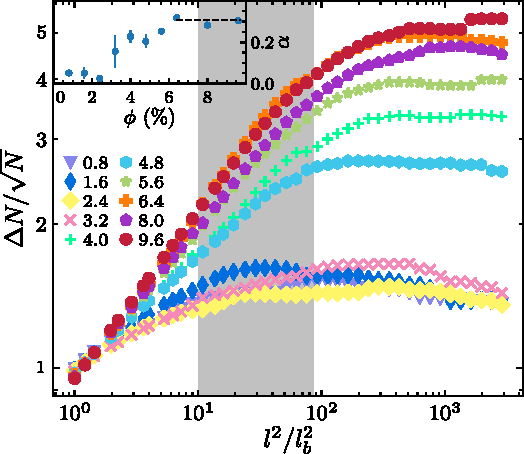
\includegraphics[width=0.47\textwidth]{figures/GNF-energy-spectra-correlation-transient/v3.pdf}
\caption[The correlation between GNF and kinetic energy and kinetic energy spectra at transient state]
{
\textbf{GNF kinetics and density flow coupling at transient state.}
(a) Kinetics of GNF at the onset of active turbulence in a $\phi=9.6\%$ suspension (legends indicates time in unit second). Inset: temporal evolution of scaling exponent $\alpha$, total kinetic energy $E$ and the area fraction of the regions with strong alignment of local velocities $M$ in the same sample.
(b) Kinetic energy and number fluctuations at corresponding time and length scales during the onset of active turbulence at volume fractions ranging from 3.6\% to 14.4\%. Black dashed line is the phenomenological fitting of the universal coupling, the same as in Fig.~\ref{fig:GNF-energy-spectra-correlation}a.
}
\label{fig:GNF-energy-spectra-correlation-transient}
\end{center}
\end{figure}

More surprisingly, we find that the same density-independent coupling also exists in the kinetic process during the transition towards bacterial turbulence. Taking the advantage of the light-powered bacteria, we trigger the onset of bacterial turbulence by suddenly turning on the light illumination on a bacterial suspension of high $\phi = XX\%$ at $t=0$ \cite{Peng2020}. The density fluctuations and the energy spectra are then monitored as a function of $t$ before the suspension reaches the steady turbulent state. Figure~\ref{fig:GNF-energy-spectra-correlation-transient} shows the temporal evolution of GNF. Different from the steady-state GNF at different $\phi$, where strong GNF persists at small length scales even for low-$\phi$ suspensions, the high-$\phi$ bacterial suspension shows no or very weak GNF at the onset of active turbulence at small $t$ with the scaling exponent $\alpha \approx XX$ at early times. The strength of GNF gradually increases over time, which leads to a smooth increase of $\alpha(t)$ (the black line in Fig.~\ref{fig:GNF-energy-spectra-correlation-transient} inset). $\alpha$ saturates to the steady state value of 0.33 above $t \approx 90$ s. Interestingly, the growth of GNF is significantly delayed compared with the formation of collective turbulent flows. Following the previous studies \cite{Cisneros2011,Peng2020}, we quantify the rise of active turbulence using the area fraction of the collective regions with strong alignment of local velocities, $M$ \cite{Liu2020}. $M$ reaches a plateau at a much earlier time around 30 s (the blue line in Fig.~\ref{fig:GNF-energy-spectra-correlation-transient} inset). The finding provides strong experimental evidence to an important prediction of the kinetic theory of active fluids \cite{Saintillan2008a,Saintillan2008b}, where density fluctuations are shown to be the nonlinear consequence of the shear stress instability and appear only at long times. At the onset of hydrodynamic instability with the emergence of the collective turbulent flow in the linear regime, particle density stays uniform with only weak fluctuations. In contrast, we find that the growth of $\alpha$ and the kinetic energy $E$ are strongly coupled and show quantitatively similar trends (the black and the orange lines in Fig.~\ref{fig:GNF-energy-spectra-correlation-transient} inset), clearly demonstrating the density-energy coupling in the kinetic process.

Lastly, we analyze the correlation between $\Delta N/\sqrt N$ and $E(k)$ during the turbulent transition for bacterial suspensions of different $\phi$ (Fig.~\ref{fig:GNF-energy-spectra-correlation-transient}b). When $\phi>\phi_c$, all the data at different $t$, $\phi$ and $l$ collapse into the same master curve obtained from the steady-state measurements \cite{Liu2020}.
This surprising result suggests that kinetic energies control not only the steady-state GNF but also the rise of GNF at each individual length scale.

\section{Conclusions}

We have conducted systematic experiments measuring density fluctuations and energy spectra of 3D bacterial suspensions over a wide range of concentrations in both the steady and transient states. The scaling behavior of the number density fluctuation $\Delta N/\sqrt N \sim N^\alpha$ observed in our experiments was in quantitative agreement with the theoretical prediction of suspensions of polar-ordered self-propelled particles. More importantly, we showed that such a scaling behavior persisted at small lengths in low-concentration suspensions well below the transition concentration to bacterial turbulence. The finding provided new experimental evidence on the existence of strong local bacterial correlation in dilute suspensions due to the long-range hydrodynamic interactions in wet 3D active fluids. In addition to density fluctuations, we also examined the energy spectra of bacterial suspensions of different concentrations. The results quantitatively verified the prediction of the energy spectra of dilute pusher-type active fluids and illustrated the emergence of the characteristic energy spectra of active turbulence with increasing concentrations in the bulk limit without the effect of confinement. Lastly, our detailed analysis of the density and velocity fields at different scales revealed a profound coupling between kinetic energy and giant number fluctuations, spanning multiple length scales from the size of single bacteria up to the size of system. Such a density-independent and scale-invariant coupling was also uncovered in the kinetic process during the transition towards bacterial turbulence. This density-energy coupling resulted in the delay of the onset of giant number fluctuations with respect to the rise of the collective turbulent flows, supporting a key prediction of the kinetic theory. As such, our study provided a comprehensive experimental benchmark on the density fluctuations and energy spectra of 3D bacterial suspensions and shed new light onto the emergent dynamics of wet active fluids.

\begin{acknowledgements}
	We thank XX, XX and XX for the help with experiments and fruitful discussions. The research is supported by NSF CBET 1702352, NSF CBET 2028652 and the Packard foundation.
\end{acknowledgements}

\bibliographystyle{apsrev4-2}
\bibliography{correlation}

\end{document}
